\documentclass{standalone}
\usepackage{etex}
\PassOptionsToPackage{rgb}{xcolor}
\usepackage{tikz}
\usepackage{pgfplots}
\usepackage{amsmath}
\usepackage{tkz-fct}  
\usepackage{makecell}
\usepackage{mathrsfs}
\usepackage{pifont}
\usepackage{textcomp}
%% set bounds here!
%%%%%%%
\newcommand{\xmax}{10}
\newcommand{\ymax}{10}
%%%%%%%%%
%\newcommand\variable_name{variable_value} %uncomment to create variables

\usetikzlibrary{shapes.geometric,arrows,backgrounds,calc,trees,decorations.pathmorphing,patterns,3d,arrows.meta,decorations.text,}
\tikzset{>={Stealth[width=1.2mm,length=1.2mm]},box/.style={draw=none,fill=none,align=center,execute at begin node=\setlength{\baselineskip}{9pt}}}
\begin{document}
\pgfplotsset{compat=1.11,axis line style={white}}
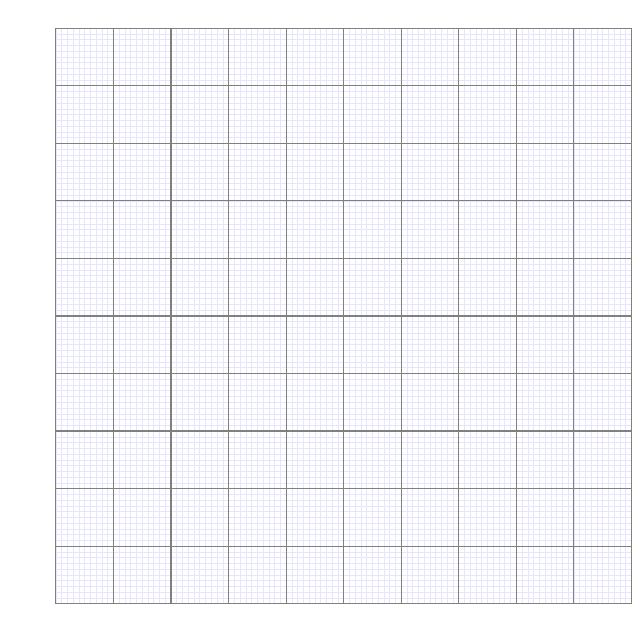
\begin{tikzpicture}
\begin{axis}[clip=false,ticks=none,xmin=0,xmax=\xmax,ymin=0,ymax=\ymax,scale mode=scale uniformly,width=3.5in, height=3.5in]

\tikz \fill [white] (0,0) rectangle (\xmax,\ymax);
\draw[help lines, step = 0.1, color = blue!10!white, very thin] (0,0) grid (\xmax,\ymax);
\draw[help lines, step = 1, color=gray] (0, 0) grid (\xmax,\ymax);


\end{axis}
\end{tikzpicture}
\end{document}